% Copyright 2004 by Till Tantau <tantau@users.sourceforge.net>.
%
% In principle, this file can be redistributed and/or modified under
% the terms of the GNU Public License, version 2.
%
% However, this file is supposed to be a template to be modified
% for your own needs. For this reason, if you use this file as a
% template and not specifically distribute it as part of a another
% package/program, I grant the extra permission to freely copy and
% modify this file as you see fit and even to delete this copyright
% notice. 

\documentclass{beamer}

% There are many different themes available for Beamer. A comprehensive
% list with examples is given here:
% http://deic.uab.es/~iblanes/beamer_gallery/index_by_theme.html
% You can uncomment the themes below if you would like to use a different
% one:
%\usetheme{AnnArbor}
%\usetheme{Antibes}
%\usetheme{Bergen}
%\usetheme{Berkeley}
%\usetheme{Berlin}
%\usetheme{Boadilla}
%\usetheme{boxes}
%\usetheme{CambridgeUS}
%\usetheme{Copenhagen}
%\usetheme{Darmstadt}
%\usetheme{default}
%\usetheme{Frankfurt}
%\usetheme{Goettingen}
%\usetheme{Hannover}
%\usetheme{Ilmenau}
%\usetheme{JuanLesPins}
%\usetheme{Luebeck}
\usetheme{Madrid}
%\usetheme{Malmoe}
%\usetheme{Marburg}
%\usetheme{Montpellier}
%\usetheme{PaloAlto}
%\usetheme{Pittsburgh}
%\usetheme{Rochester}
%\usetheme{Singapore}
%\usetheme{Szeged}
%\usetheme{Warsaw}
\usepackage{hyperref}
\usepackage{multicol}

\title{Stealth File Systems for Proactive Forensics Support in Custom Android ROMs}

% A subtitle is optional and this may be deleted
%\subtitle{Optional Subtitle}

\author{Guide: Dr. Prabhaker Mateti\inst{1} \and Sudip Hazra\inst{2}}
% - Give the names in the same order as the appear in the paper.
% - Use the \inst{?} command only if the authors have different
%   affiliation.

\institute[Universities of Somewhere and Elsewhere] % (optional, but mostly needed)
{
  \inst{1}%
  Wright State University
  \and
  \inst{2}%
  Amrita Centre For Cyber Security Systems and Networks\\
 Amrita University}
% - Use the \inst command only if there are several affiliations.
% - Keep it simple, no one is interested in your street address.

\date{13 March 2017}
% - Either use conference name or its abbreviation.
% - Not really informative to the audience, more for people (including
%   yourself) who are reading the slides online

\subject{Theoretical Computer Science}
% This is only inserted into the PDF information catalog. Can be left
% out. 

% If you have a file called "university-logo-filename.xxx", where xxx
% is a graphic format that can be processed by latex or pdflatex,
% resp., then you can add a logo as follows:

% \pgfdeclareimage[height=0.5cm]{university-logo}{university-logo-filename}
% \logo{\pgfuseimage{university-logo}}

% Delete this, if you do not want the table of contents to pop up at
% the beginning of each subsection:
\AtBeginSubsection[]
{
  \begin{frame}<beamer>
   \begin{multicols}{3}
     \tableofcontents[currentsection,currentsubsection]
   \end{multicols}
  \end{frame}
}

% Let's get started
\begin{document}

\begin{frame}
  \titlepage
  \centering
 
  \begin{figure}
  \centering
 \vspace{-.5cm}
  
\includegraphics[width=.3\textwidth,height=.3\textheight]{images/AVV_colour}
  
  \end{figure}
  
 
\end{frame}

\begin{frame}{Outline}
  
  \begin{multicols}{3}
    \tableofcontents
  \end{multicols}
  
\end{frame}

% Section and subsections will appear in the presentation overview
% and table of contents.
\section{Introduction}

\subsection{Why Android}
\begin{frame}{Why Android}{Mobile OS Market}
\begin{figure}
\centering
\caption{Smartphone OS Market Share, 2016 Q2
}
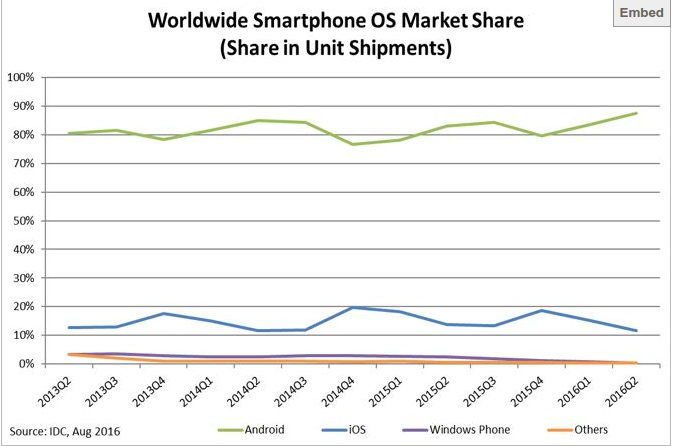
\includegraphics[width=.6\textwidth,height=.5\textheight]{images/idc}
\label{imageLabel}
 \scriptsize{Source:http://www.idc.com/prodserv/smartphone-os-market-share.jsp}
\end{figure}

  
\end{frame}
\subsection{Why Mobile Forensics is Important}
\begin{frame}{Why Mobile Forensics is Important}
The use of cell phones and computers are like a journal or diary of users’ lives. Just from cell phones, a mobile phone forensic analysis by International Investigators can reveal a great deal of data, including:

\begin{itemize}
\item Dialed, incoming and missed calls (history logs)
\item Text messages
\item Instant message activity
\item Email
\item Internet activity including search histories
\item Phone location information (using GPS) and cell phone tower triangulation
\end{itemize}
\end{frame}
\subsection{Problem Scenario}
\begin{frame}{Problem Scenario}
To Catch a Thief, Think Like a Thief!
\begin{itemize}
\item If criminals and crime organizers use smart phones, what would they do?
\item Will they browse? If so which browser? What site?
\item How to predict the next move?
\item How to Collect Evidence if they erase the Phone Memory aka. Factory Reset.
\end{itemize}
\end{frame}

\section{Background}
\subsection{Types of Mobile Forensics Investigation}
\begin{frame}{Types of Mobile Forensics Investigation}
\begin{itemize}
\item \textbf{Reactive Forensics :}\\
Investigation done after Crime has happened.Susceptible to Applications like Uninstall-It, can potentially wipe out all user data and Device Encryption can be a barrier for investigation.

\item \textbf{Proactive Forensics:}\\
A suspect or potential terrorist is monitored proactively in realtime to prevent a crime.
Real-time monitoring and analysis is possible.
Data Encryption will not be a hindrance in evidence collection.Ability to retrieve deleted data and logs and prevent potential crimes .
\end{itemize}
\end{frame}

\subsection{Forensic Support Framework}
\begin{frame}{Forensic Support Framework}

\begin{figure}
\centering
\caption{Features of forensic Rom developed by Aiyappan Et.al \cite{Aiyappan}  and Karthik Et.al \cite{Karthik} }
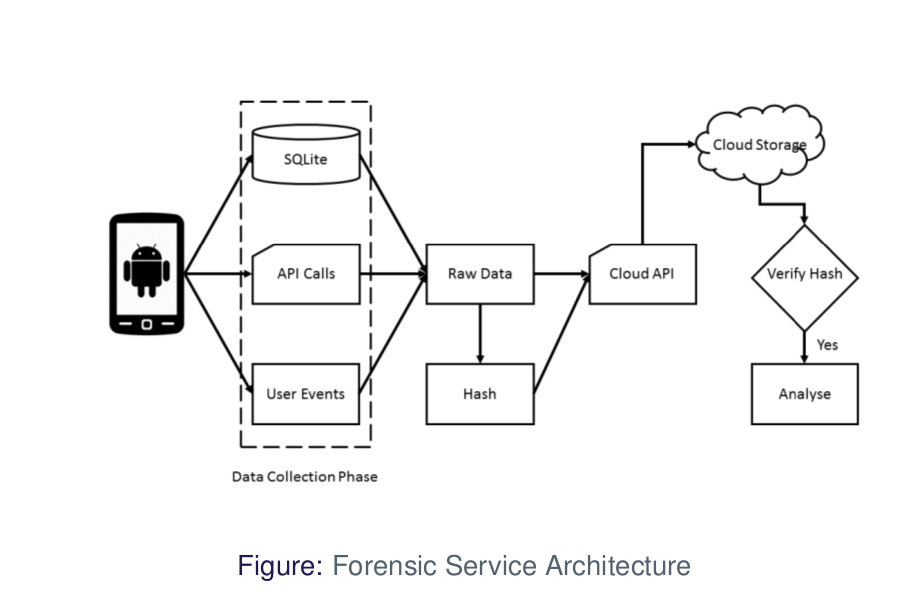
\includegraphics[width=.6\textwidth,height=.4\textheight]{images/forensic}

\label{imageLabel}
 \end{figure}
 \small 1 .Captures All User Activities.\\
 \small 2 .Key-logging and Call  Tapping 		 Facility.\\
\small  3 .Opportunistically Uploads In Cloud.\\
\small  4. Hiding the Process using hidepid =2.\\
\small  5. Data Stored in /forensic partition only accessible to Root.\\
 
\end{frame}
\subsection{Shortfalls}
\begin{frame}{Shortfalls}

	\begin{itemize}
	
	\item{
	
	What if The Suspect Roots the Phone ?
	}
	\bigskip
	\item{
	
		Can Find the /forensic Partition.	
	}	
	\end{itemize}

\end{frame}
\subsection{Possible Solutions}
\begin{frame}{Posible Solutions}
	\begin{itemize}
	\item{
	Encrypting The /forensic partition can Still arise Suspicion.
	}
	\bigskip
	\item{
	Creating A Fuse File System and enable Stealth Features and Copy all Forensically Relevant Data in that File System.
	
	}
	\end{itemize}
\end{frame}
\subsection{File System in User Space}
\begin{frame}{File System in User Space}
\begin{itemize}
\item{
The Filesystem in Userspace (FUSE) is a special part of the Linux \indent kernel that \indent allows regular users to make and use their own file-systems \indent without needing to change the kernel or have Root privileges.
}

\begin{figure}
\centering
\caption{A Fuse Filesystem.}
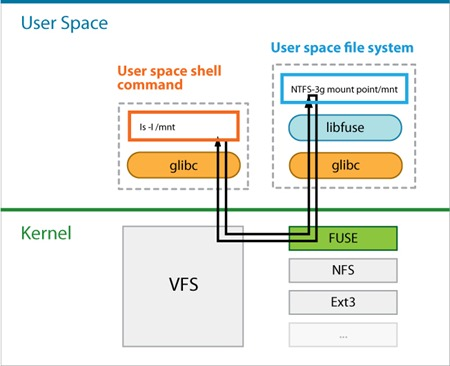
\includegraphics[width=.6\textwidth,height=.5\textheight]{fuse}
\label{imageLabel}
\scriptsize{Source:en.wikipedia.org/wiki/Filesystem in Userspace}
\end{figure}
\end{itemize}
\end{frame}

\subsection{Cloud File System}
\begin{frame}{Cloud File System}
	\begin{itemize}
	\item{Using FUSE we can mount Cloud Drive in Our System and Use it Like a Local File System.
	}
	\bigskip
	
	 \item \href{https://github.com/GoogleCloudPlatform/gcsfuse}{Gcsfuse:} A user-space file system for interacting with Google Cloud Storage.
	 \bigskip
	 
	 \item \href{http://www.archiware.com/products/wingfs}{Wingfs:} A debian Package to mount various cloud storage drives as user-space file systems.
	 \bigskip 
	 \item \href{https://ahmetalpbalkan.com/blog/introducing-azurefs/}{Azurefs:} A python package to mount Azure blob storage as Local File system.
	 \end{itemize}	   	
\end{frame}

\section{Problem Definition}
\begin{frame}{Problem Definition}{What is the Goal}
\begin{itemize}
\item To mount the Cloud storage as a Local File system in Android.
\item To Provide Support for Multiple Cloud storage Providers.
\item The forensic file system will copy itself in parts to the cloud file system.
\item The file system will be opportunistically get uploaded to the cloud storage.

\item To hide both the Cloudfs and the forensic partition using Rootkits.
\end{itemize}
\end{frame}
\section{Solution Outline}
\begin{frame}{Architecture Diagram}
Here we propose a Stealth File system with cloud support Below the Android Software
stack.
\begin{figure}
\centering

\includegraphics[width=.7\textwidth,height=.6\textheight]{images/FUSE}
\caption{Android Cloud Storage Service}
\label{imageLabel}
\end{figure}
\end{frame}
\subsection{Modules}
\begin{frame}{Modules}{Stealth File Systems}
\begin{itemize}
\item The stealth file system will be a seperate file system which will be used by the forensic service to
copy all the forensically relevant data from the relevant device partitions like /data to the stealth
file system.
\item  The stealth file system will be based on ext4 file systems, rootkits will be used to hide
the file volumes from commands like df and du. \item The rootkit will also hide the forensic service
running in the background by hooking on to the sys\_call\_table and filtering out the output. 

\end{itemize}
\end{frame}
\begin{frame}{Modules}{Cloud File System}
\begin{itemize}
\item The cloud File system will made using fuse , and we will be able to localy mount a cloud drive
as the cloud file system. It will support various cloud providers using api’s
\item \textbf{As per the official android documentation the external storage (SD cards) are accessed by the
Android system using FUSE which implies that FUSE is supported by the kernel directly so we
dont need to add fuse support in kernel.}
\end{itemize}
\end{frame}
\subsection{Cloud Storage API's}
\begin{frame}{Cloud Storage API's}
\textbf{Cloud Storage API's Examples:}\\
Dropbox Cloud Storage Api's:\\
1 .Create a Dropbox folder 
\bigskip
post('https://api.dropbox.com/1/fileops/create\_folder', args)\\

2.Rename a Dropbox file/directory object.
\bigskip
post('https://api.dropbox.com/1/fileops/move', args)

3.Delete a Dropbox file/directory object.
\bigskip
post('https://api.dropbox.com/1/fileops/delete', args)\\
4.Get Dropbox metadata of path.
\bigskip
get('https://api.dropbox.com/1/metadata/auto' + path, args)


\end{frame}
\subsection{Calling Native Libraries Using Java}
\begin{frame}{Calling Native Libraries Using Java}
Since libfuse is a native library written in c, We need to have some wrapper functions to call the Native Libraries in Java.\\
\bigskip
This can be achieved by :\\
\bigskip
1.Java Native Interface(JNI).\\
\bigskip
2.Java Native Access(JNA).\\
\bigskip
3.Java Native Runtime(JNR).\\

\end{frame}
\subsection{Calling Native Code using JNA}
\begin{frame}{Calling Native Code using JNA}
Package net.fusejna.examples;

import java.io.File;\\
import java.nio.ByteBuffer;\\
import net.fusejna.DirectoryFiller;\\
import net.fusejna.ErrorCodes;\\
import net.fusejna.FuseException;\\
import net.fusejna.StructFuseFileInfo.FileInfoWrapper;\\
import net.fusejna.StructStat.StatWrapper;\\
import net.fusejna.types.TypeMode.NodeType;\\
import net.fusejna.util.FuseFilesystemAdapterFull;\\
\bigskip
We need to Subclass net.fusejna.FuseFilesystem and override the methods we need i.e FuseFilesystemAdapterFull.\\
\bigskip

public int readdir(final String path, final DirectoryFiller filler)\\
	{
		filler.add(filename);
		return 0;
	}
\end{frame}

\subsection{Addressing Performance Issues}
\begin{frame}{Addressing Performance Issues}
Android imposes user-level filesystem (FUSE) over native filesystem partition to provide flexibility in managing the internal storage space and to maintain host compatibility. However, the overhead of user-level filesystem is prohibitively large and the native storage bandwidth is significantly under-utilized.
In order to address this overhead of user-level filesystem and Compensate the JNA Overhead.We will be using Buffered Fuse\cite{jeong2014buffered}\\
\bigskip
The key technical ingredients of Buffered FUSE\cite{jeong2014buffered} are\\
(i) extended FUSE IO size.\\
(ii) internal user-level write buffer (FUSE buffer).\\
(iii) independent management thread which performs time driven FUSE buffer synchronization.
\end{frame}

\bigskip

\bigskip
In this paper\cite{jeong2014buffered} the author has increased the fuse buffer size to 512 kb and FUSE Buffer , also the android ioschdedular has been changed and file system has been changed to XFS. They are claiming 70 \% increase in speed.The modified sdcard.c has the following changes on study:\\
In android/platform\_system\_core/sdcard.c:\\
They have defined a FUSE CACHE.\\

\#include pthread.h\\
\#define FUSE\_CACHE 1\\ 
 \#define FUSE\_CACHE\_THREAD 1 \\
 \#define FUSE\_CACHE\_SIGNAL 0 \\
 \#define FUSE\_IO\_SIZE 512*1024\\
\#define FUSE\_CACHE\_SIZE FUSE\_IO\_SIZE*4\\
\#define FUSE\_CACHE\_NUM 4\\


\subsection{Stealth}
\begin{frame}{Stealth\cite{doar-e}}
\begin{itemize}
\item The vector table is a table that actually contains control transfer instructions that jump to the respective exception handlers.\\

\item On 32-bit ARM Linux this address is 0xffff0000.\\
\item Our plan is going to be to backdoor the kernel by overwriting the SWI exception vector with code that jumps to our backdoor code. This code will check for a magic value in a register and if it matches, it will elevate the privileges of the calling process.\\
\item If we choose an appropriate location in kernel space, our code will exist as long as the machine is running

\end{itemize}
\end{frame}







\section{Implementation}
\begin{frame}{Implementation}
Compiled Android kernel with module support
\begin{itemize}
\item Android kernel, by default do not support loadable modules. 
\item make ARCH=arm goldfish\_defconfig (This will create our .config)
\item Edit the .config file and searched for the line “CONFIG\_MODULES”
It was unset for me and the line looked liked this
\item CONFIG\_MODULES is not set
I changed the line to CONFIG\_MODULES=y, saved and closed the file.
\item Now, the command to build the kernel
make ARCH=arm CROSS\_COMPILE=~/Desktop/mydroid/prebuilt/linux-x86/toolchain/arm-eabi-4.4.3/bin/arm-eabi-


\end{itemize}
\end{frame}



\section{Summary}
\begin{frame}{Summary}
  \begin{itemize}
  \item
    \alert{Process Hiding} can also be Implemented Using this Technique
  \item
    The \alert{Stealth File-system}  will periodically copy the forensically relevant data from the normal file system
  \item This data will be moved to the \alert{Mounted Cloud Drive} and opportunistically uploaded to the cloud server. 
  \end{itemize}
  
 
\end{frame}


\begin{frame}{Summary}
\begin{block}{Summary}
This Framework can effectively Hide the forensic as well as the cloud file system so that even if the Suspect is connecting to adb to check the internal state , He will not be able to find the  hidden File systems.
\end{block}


\end{frame}

% Placing a * after \section means it will not show in the
% outline or table of contents.



% All of the following is optional and typically not needed. 
\appendix
\section<presentation>*{\appendixname}
\subsection<presentation>*{Reference}

\begin{frame}[allowframebreaks]
  \frametitle<presentation>{References}
  
  \begin{thebibliography}{10}
  \bibitem{Aiyappan} 
  \textit{Android forensic support framework},
  Aiyappan.P
  Advisor:Prabhaker Mateti,
  M.Tech thesis, Amrita
  Vishwa Vidyapeetham,2015
   
  \bibitem{Karthik} 
  \textit{Proactive Forensic Support for Android Devices},
  Karthik K. 
  Advisor:Prabhaker Mateti
  M.Tech thesis,
  Amrita Vishwa Vidyapeetham,2016 
  
  \bibitem{Dong}
    \textit{Android platform based linux kernel rootkit},
    Dong-Hoon You, Bong-Nam Noh,
    Malicious and Unwanted Software (MALWARE), 2011 6th International Conference ,IEEE
    
    \bibitem{jeong2014buffered}
      \textit{Buffered FUSE: optimising the Android IO stack for user-level filesystem},
	  Jeong, Sooman and Won, Youjip,
      International Journal of Embedded Systems,2014.
      
      \bibitem{doar-e}
      \textit{Corrupting the ARM Exception Vector Table},
      http://doar-e.github.io/blog/2014/04/30/corrupting-arm-evt/
      
    
    
    
    
    
    
 
  
   
 
  \end{thebibliography}
  
  
   
\end{frame}

\end{document}


